\chapter{Background}
\label{ch:background}

\section{Understanding Continuity Anomalies}

\subsection{Definitions and guidelines}

Before proceeding with the discussion of continuity in film, let's establish the following:

Frame is a single static image captured by the camera. Displayed sequentially at a usual standard rate of 24 frames per second, it creates the perception of continuous motion.

Take is a single video recording from the moment the camera starts rolling until it stops. Typically multiple takes of the same action are filmed to capture the best possible shots and to provide coverage from different camera angles required for the scene.

Shot is a continuous sequence of frames, retrieved from the take. It serves as a distinct segment between cuts in the final edit, forming a scene.

Scene consists of multiple shots usually set in the same location and time, representing a distinct narrative moment within the film.

Continuity encompasses a wide range of visual and narrative details that should remain consistent across a scene. There are established guidelines in the industry that help maintain it~\cite{miller1999}. For example, a well-known continuity rule is where clocks, watches, or phone displays in a scene must show the same time across different shots if they represent the same narrative moment. Another common rule is to match eyelines between shots to ensure that the character's gaze aligns correctly with whatever or whoever they are looking at. In the video for VanityFair~\cite{vanityfair2023} Martin Scorsese's long-time script supervisor Martha Pinson showcased a few of the main things she looks out for in a film (see Figure 2.1).

\begin{figure}[h]
\centering
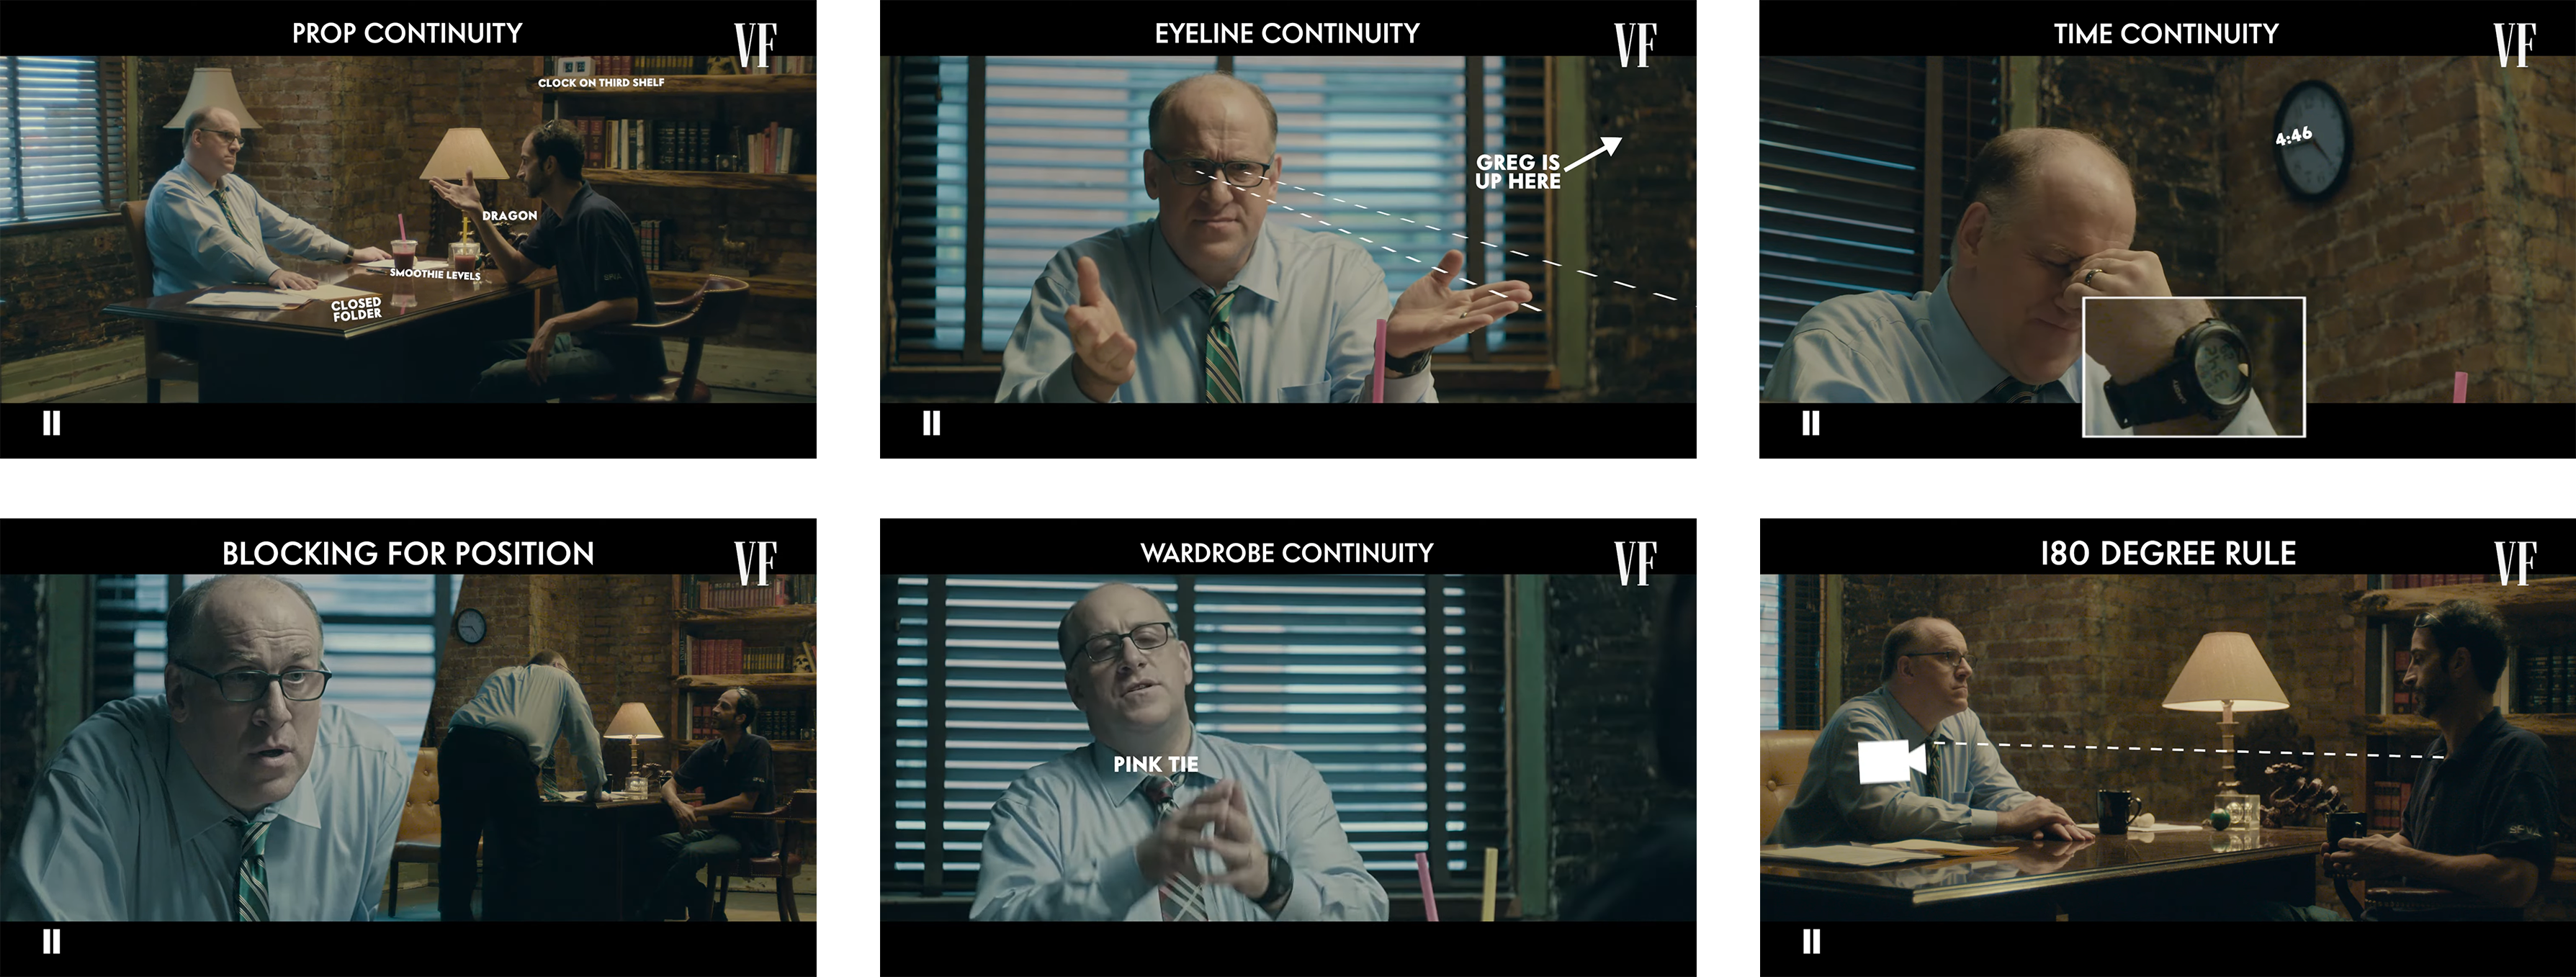
\includegraphics[width=0.8\textwidth]{figures/VF-Continuity.png}
\caption{Examples of continuity rules monitored by script supervisors. Top row (left to right): prop continuity, eyeline continuity, time continuity. Bottom row (left to right): blocking for position, wardrobe continuity, 180-degree rule. Source:~\cite{vanityfair2023}}
\label{fig:continuity-examples}
\end{figure}

\subsection{Variation in continuity errors}

Pat P. Miller in his book "Script Supervising and Film Continuity" defines it as "the art and craft of maintaining consistency in every visual and aural detail from shot to shot"~\cite{warm2008}. This definition encompasses multiple error categories requiring different detection approaches. Table 2.1 categorises these error types with their characteristics and typical manifestations.

\begin{table}[h]
\centering
\begin{tabularx}{\textwidth}{|l|X|X|}
\hline
\textbf{Error Type} & \textbf{Description} & \textbf{Common Examples} \\
\hline
Temporal Continuity & Inconsistent time progression within scenes that should represent continuous action & 
\begin{itemize}[nosep,leftmargin=*]
\item Clock faces showing impossible time jumps
\item Candle lengths increasing between shots
\item Daylight changes within supposedly continuous action
\item Weather variations during single conversations
\end{itemize} \\
\hline
Spatial Continuity & Incorrect object placement and positioning between shots & 
\begin{itemize}[nosep,leftmargin=*]
\item Props appearing or disappearing between shots
\item Costume elements changing state (buttons, zippers, accessories)
\item Character positions jumping unnaturally
\item Background elements shifting location
\end{itemize} \\
\hline
Action Continuity & Broken physical movement flow across edits & 
\begin{itemize}[nosep,leftmargin=*]
\item Gestures not matching across cuts
\item Objects held in different hands
\item Incomplete actions (drinking, smoking, eating)
\item Mismatched movement directions
\end{itemize} \\
\hline
Technical Continuity & Unintended production elements visible in final footage & 
\begin{itemize}[nosep,leftmargin=*]
\item Crew reflections in surfaces
\item Equipment visible in frame
\item Lighting inconsistencies
\item Focus or exposure jumps
\end{itemize} \\
\hline
\end{tabularx}
\caption{Classification of continuity errors in film production with descriptions and common examples}
\label{tab:continuity-errors}
\end{table}

\section{The Cognitive Science of Continuity Supervision}

\subsection{Vigilance Task Characteristics}

Script supervision exemplifies a sustained vigilance task, a category extensively studied in cognitive psychology. Warm, Parasuraman and Matthews demonstrated that vigilance tasks impose significant cognitive load, with performance typically declining 10–30\% within the first 30–60 minutes of sustained attention~\cite{see1997}. This 'vigilance decrement' occurs across diverse monitoring tasks, from radar operation to quality-control inspection. Film production amplifies these challenges through several factors:

Extended duration: Production days typically span 10–14 hours, far exceeding experiment designs of laboratory vigilance studies. Script supervisors must maintain attention across this entire period, often with minimal breaks between setups.

Information overload: Modern 4K cameras capture 8.3 million pixels per frame at 24–30 frames per second. In this data stream, supervisors track dialogue delivery, actor positions, prop placement, wardrobe details and temporal elements simultaneously. This can be overwhelming to track for one supervisor.

Low signal prevalence: Actual continuity errors occur relatively rarely. Signal-detection theory predicts that low target prevalence shifts response criteria, increasing miss rates. When errors are uncommon, maintaining sensitivity becomes cognitively demanding.

Working memory taxation: Non-linear shooting schedules require supervisors to maintain mental models of narrative chronology while observing out-of-sequence filming. This dual-task paradigm markedly affects detection performance.

Script supervisors use various mitigation strategies including photographic documentation, detailed notes and systematic checking procedures to reduce error rates~\cite{grier2003}.

\section{Film Production Workflows}

\subsection{Production Constraints}

Understanding production workflows proves essential for system design. Film sets operate on carefully orchestrated schedules where delays cascade expensively. Whereas simple changes to a set can take just a few minutes, larger-scale lighting or camera adjustments can take up to half an hour; on average, a regular reset between takes is about 5 minutes. These windows define the timeline in which continuity anomalies are usually corrected and another set of notes is recorded. A system requiring too long to process the footage on a small production with short reset periods would miss the prevention opportunities, rendering it impractical.

\subsection{Tools and Practices}

Script supervisors currently employ a hybrid analogue–digital workflow that combines modern technology with traditional methods (see Figure 2.2). Digital systems, particularly ScriptE~\cite{scriptesystems2024}, have become the dominant tool in professional productions, providing iPad-based interfaces that enable supervisors to log takes, track coverage and annotate scripts efficiently. However, these systems lack automated error-detection capabilities, requiring supervisors to rely entirely on manual observation.

Additionally, supervisors use digital cameras extensively to capture reference images for each setup, creating comprehensive visual documentation of props, wardrobe, makeup, actor positions and set arrangements~\cite{scriptation2025}. This multi-tool approach extends to team coordination, where supervisors must communicate with multiple departments including costume, props and makeup. Each department maintains its own continuity records, which creates beneficial redundancy but also introduces the potential for inconsistencies across documentation systems.

\begin{figure}[h]
\centering
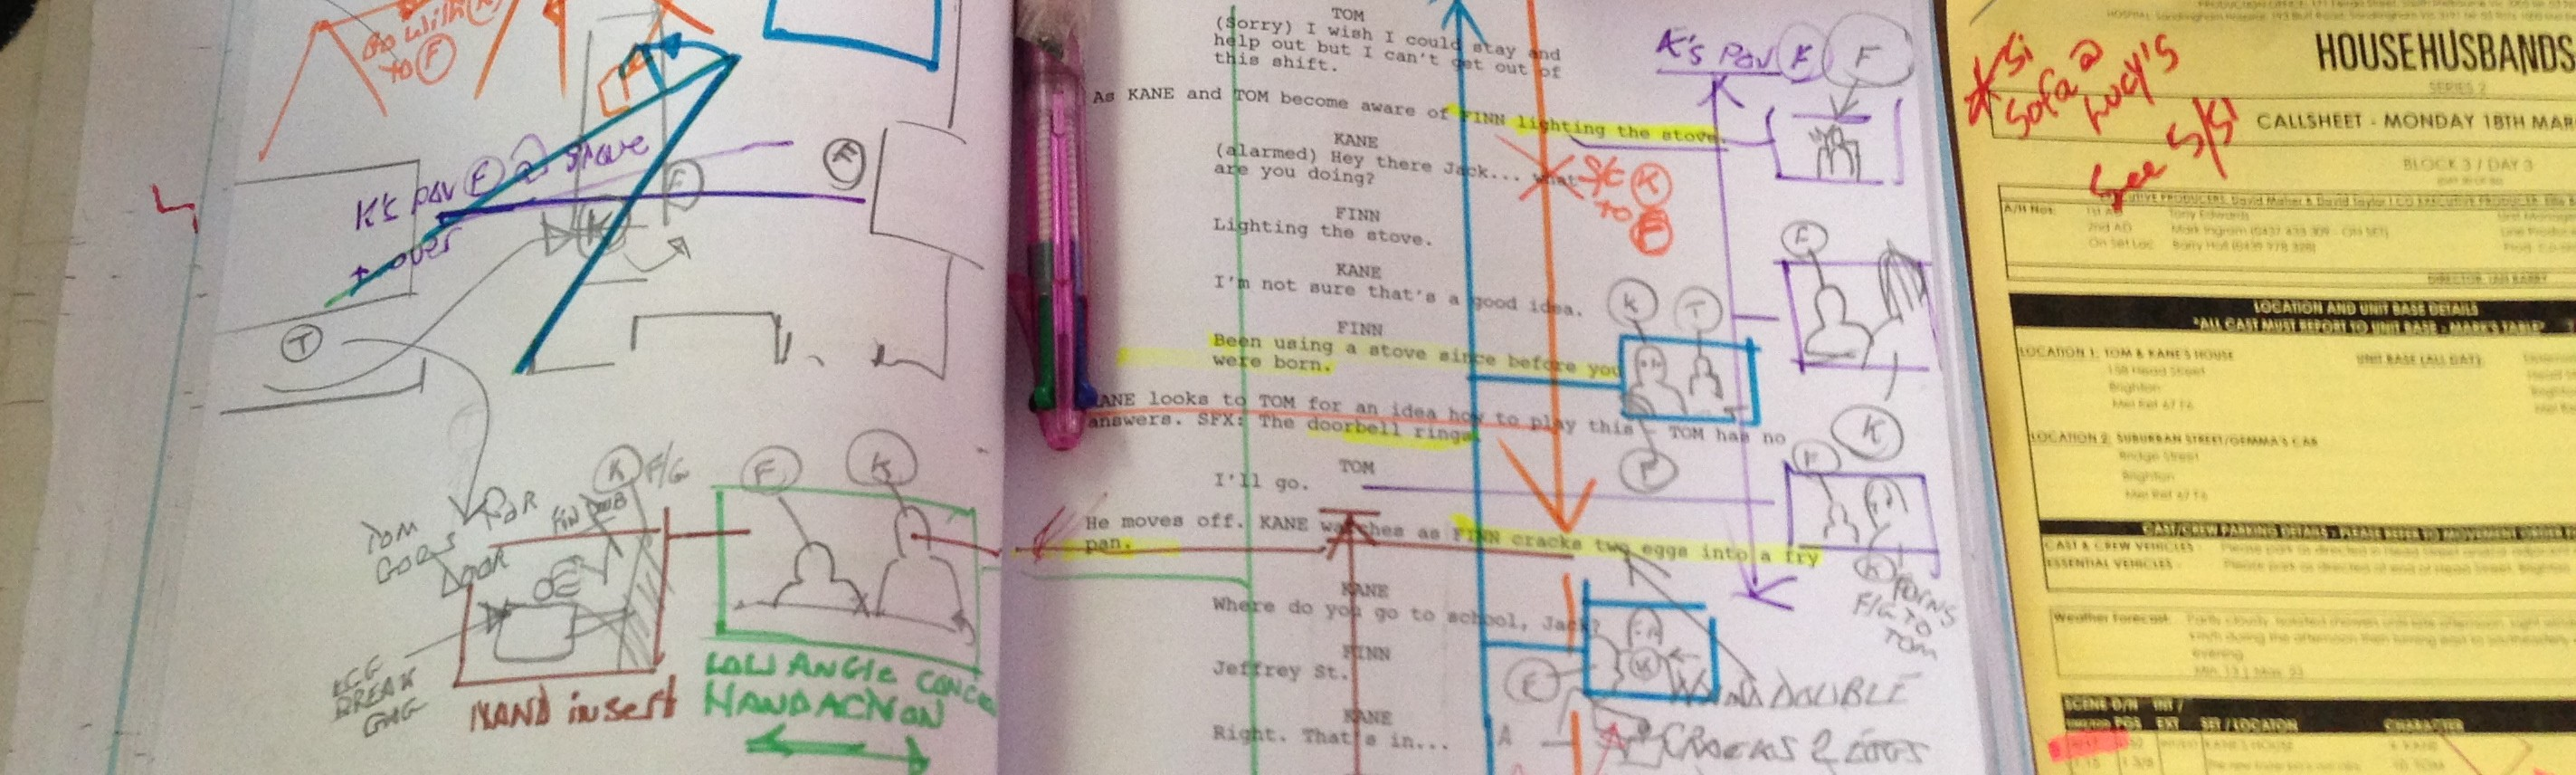
\includegraphics[width=0.8\textwidth]{figures/script_annotations.jpg}
\caption{Annotated script and notes on set of House Husbands~\cite{mskemosabi2013}}
\label{fig:script-notes}
\end{figure}

\subsection{From the Perspective of Script Supervisors}

Script supervisors enter the production pipeline 4–8 weeks before principal photography, conducting comprehensive script breakdowns that identify continuity elements, perform timing analysis, and create department-specific documentation. This pre-production phase produces the continuity master reference detailing costume changes, prop states, and temporal progressions across the narrative timeline. During filming, script supervisors arrive 30–60 minutes before crew call to coordinate daily continuity requirements. Positioned in video village, they document every take with technical camera data, timing information, and continuity observations whilst generating three essential documents: lined scripts showing coverage patterns, editor's logs detailing each take, and daily progress reports distributed within two hours of wrap.

Post-production responsibilities commence immediately after wrap, requiring 1–2 weeks to compile the production book containing all continuity documentation, lined scripts, and editorial notes. Script supervisors then remain available for 4–6 weeks of consultancy, resolving continuity questions during editing and providing specifications for potential reshoots. Their formal responsibilities conclude upon delivery and acceptance of all materials by the post-production team, though complex productions may retain them throughout editing to ensure narrative coherence~\cite{wickens2015,kreativalchemy2024}.

\section{Computer-Vision Capabilities and Limitations}

\subsection{Object Detection}

Modern object-detection systems follow two main approaches. Single-stage detectors examine entire images in one pass to find objects, a good example of such is the YOLO (You Only Look Once) family. YOLOv11 represents one of the latest iterations, which introduces architectural improvements including C3k2 (Cross Stage Partial with kernel size 2) blocks, which enhance feature extraction whilst reducing computational load, and parallel spatial attention mechanisms that help the model focus on relevant image regions. YOLOv11 achieves 54.5\% mAP on the COCO dataset whilst maintaining inference speeds of 13.5 milliseconds, making it suitable for real-time applications~\cite{ultralytics2024}. Recent comparative studies demonstrate that the YOLO series consistently balances speed and accuracy across different hardware configurations, with newer versions showing significant improvements in detecting smaller objects, which can be critical for video analysis tasks~\cite{khanam2024}.

Two-stage detectors take a different approach by first identifying regions likely to contain objects, then classifying those regions. Meta's Detectron2 framework implements this methodology through a modular design supporting various backbone networks~\cite{lv2023}. When configured with Mask R-CNN and ResNet-50-FPN, Detectron2 achieves 41.0\% box AP and 37.1\% mask AP on COCO (Common Objects in Context), prioritising accuracy over speed. This framework has proven particularly effective in medical imaging applications, achieving 99.3\% accuracy in diabetic retinopathy lesion detection~\cite{premiumbeat2023}. The modular architecture allows researchers to adapt components for specific requirements, such as tracking objects across video frames or detecting partially occluded items.

The choice between architectures depends on application requirements. Single-stage detectors excel in scenarios demanding immediate response, for example, autonomous vehicles require sub-20ms detection for safe navigation. Two-stage detectors are more suitable for applications that allow longer processing times, such as medical diagnosis or forensic video analysis where accuracy outweighs speed constraints. Recent developments in transformer-based models like DETR (DEtection TRansformer) begin to blur the traditional distinction between single-stage and two-stage detectors~\cite{carion2020}. However, traditional architectures remain dominant in production deployments due to their established performance characteristics and extensive optimisation for various hardware platforms.

\subsection{Semantic Understanding Gap}

The fundamental challenge lies not in detecting objects but understanding their narrative significance. Consider a coffee cup that appears half-full in one shot and empty in the next. Object detection easily identifies the cup's presence and even how full it is through segmentation. However, determining whether this change represents a continuity error (cup state changed incorrectly), intentional storytelling (character drank between shots) or an acceptable variation (minimal story impact) through semantic reasoning is beyond current computational capabilities. Nevertheless, the rapid advancement of Multimodal Large Language Models (MLLMs) promises to enable accurate image-to-text analysis. These models are already being deployed in complex applications, including semantic correction within text-to-image diffusion systems~\cite{tan2020}. At present, however, such models exhibit limitations in spatial reasoning, object recognition, numerical accuracy, and fine detail perception.

\subsection{Applicable Techniques}

Despite limitations in semantic understanding, several computer vision techniques show particular promise for continuity detection in film production:

Co-attention mechanisms for implicit correspondence: The COAM (Co-Attention Module) architecture enables automatic alignment between image pairs by computing cross-attention between feature maps. Each feature vector at location $(x_1, y_1)$ in the first image attends to all locations in the second image, creating spatially warped features that effectively register the images without explicit transformation computation. This approach achieves 60.7\% accuracy on change detection benchmarks whilst maintaining real-time performance at 6.37 seconds per frame pair~\cite{zhang2023}.

Siamese U-Net architecture with change detection heads: A dual-stream encoder processes image pairs simultaneously, extracting multi-scale features that are then cross-attended and decoded back to full resolution. The architecture concludes with a CenterNet detection head that produces bounding boxes around changed regions, effectively framing change detection as an object detection problem rather than pixel-wise segmentation. This design choice significantly reduces post-processing requirements whilst maintaining high localisation accuracy~\cite{zhang2023}.

Spatial Transformer Networks for geometric normalisation: STNs learn to predict homography parameters that transform cropped objects to canonical views, crucial for handling viewpoint variations in film shots. When applied to analogue clock reading, this alignment step improved recognition accuracy by 14.3\% on real-world data, demonstrating the importance of geometric normalisation even when objects appear at arbitrary angles or positions within the frame~\cite{ma2024}.

Time prediction through multi-class classification: Rather than regression-based approaches, treating time reading as a 720-way classification problem (12 hours × 60 minutes) provides more robust predictions. This discrete formulation naturally handles the circular nature of time and allows the network to learn common time patterns. Combined with pseudo-labelling techniques that exploit temporal uniformity in videos, this approach achieves 82.9\% accuracy without manual annotations~\cite{ma2024}.

PaddleOCR's DBNet for real-time text detection: The Differentiable Binarisation Network uses a learnable threshold map alongside the probability map to produce sharp text boundaries, achieving 80\% F-score at 8.7 FPS. Its modular design supports multiple recognition backends including CRNN and STAR-Net, making it adaptable for detecting various text elements within scenes~\cite{kuang2021}.

\section{Related Work Analysis}

\subsection{Pickup and Zisserman (2009)}

The sole directly relevant prior work, 'Automatic retrieval of visual continuity errors in movies'~\cite{pickup2009}, pioneered computational approaches to continuity detection. Their methodology:

\begin{itemize}
\item Detected shots using RGB histogram differences between consecutive frames
\item Matched shots from similar viewpoints using L1 histogram distances
\item Registered frame pairs using homography estimation with RANSAC
\item Excluded human regions using upper-body HOG detectors
\item Computed pixel-wise differences between registered frames
\item Ranked shots by the number of unexplained discrepancy pixels
\end{itemize}

Whilst Pickup and Zisserman's approach established foundational concepts for computational continuity detection, a few critical limitations prevent it from being applicable in production workflows. Most significantly, their system operates exclusively on fully edited sequences. It necessitates completed post-production before analysis even begins, which defeats the purpose of prevention-based continuity supervision. The evaluation methodology also presents concerns: whilst the paper successfully demonstrates retrieval of known errors from specific films, it lacks comprehensive accuracy metrics. Despite these limitations, the underlying design principles: shot matching through viewpoint similarity, geometric registration and human-aware exclusion zones retain conceptual validity. These techniques, reimplemented with modern architectures, could potentially address the real-time continuity monitoring challenge that the original work could not achieve.

\subsection{Adjacent Research Domains}

Computer Vision in Film Analysis: Schmidt et al.~\cite{schmidt2021} demonstrated that sampling films at one frame per second provides sufficient temporal resolution for narrative analysis. Their study applied object detection, emotion recognition, and demographic prediction to five canonical films, successfully identifying significant differences between genres and temporal patterns. This sampling rate aligns with our continuity detection requirements, as continuity errors persist across multiple seconds rather than occurring frame-by-frame. Their finding that object detection can reveal recurring motifs, such as clocks in Metropolis, suggests similar techniques could identify continuity-relevant objects across shots.

Sports Analytics and Tracking: Modern sports analytics employs transformer-based architectures for real-time multi-player tracking. SoccerNet-Tracking achieves 71.5\% HOTA (Higher Order Tracking Accuracy) with the ByteTrack algorithm across multiple camera views~\cite{cioppa2022}. The system tracks 22 players simultaneously at 25 fps. Recent basketball tracking systems incorporate deep learning models to predict player movements, with trajectory prediction achieving high accuracy for short-term horizons~\cite{hauri2022}. These advances demonstrate robust object tracking under rapid motion and occlusion. However, sports systems operate within constrained environments with fixed camera positions, advantages that might be unavailable in dynamic film sets.

Manufacturing Quality Control: Automated visual inspection systems have revolutionised defect detection in manufacturing, with state-of-the-art methods achieving detection rates exceeding 99\% for surface defects. Recent approaches like PatchCore achieve >99\% AUROC on the MVTec industrial anomaly detection dataset~\cite{farid2016}. Deep learning systems can identify defects as small as 0.02 mm² on high-speed production lines~\cite{wang2004}. This domain's emphasis on detecting subtle deviations from expected patterns directly parallels continuity error detection. Manufacturing systems excel at identifying 'what should not be there', precisely the challenge when attempting to detect misplaced props or costume changes between takes.

Autonomous Vehicle Perception: Current autonomous driving systems process visual data at unprecedented scales. Waymo's 5th generation perception stack utilises 5 LiDAR units and 29 cameras, processing millions of 3D points per second~\cite{waymo2020}. The Waymo Open Dataset demonstrates the scale of modern autonomous perception, containing over 12 million 3D bounding box annotations across diverse driving conditions~\cite{sun2020}. The domain's expertise in handling varying weather conditions, occlusions, and multi-object tracking provides methodological insights. Particularly relevant is the use of temporal fusion techniques that aggregate information across multiple frames to improve detection reliability. However, these computational capabilities far exceed film production requirements.

\section{Summary}

The background analysis reveals a complex problem at the intersection of cognitive science, film production and computer vision. Human limitations in sustained vigilance tasks create genuine need for automated assistance. Current production workflows provide integration opportunities in natural reset windows. Although computer vision has achieved remarkable capabilities, the semantic understanding required for continuity detection remains challenging. The absence of prior research, despite a clear industry niche, highlights both the difficulty and opportunity this problem presents.